\documentclass[aspectratio=169,10pt]{beamer}
\usepackage[T1]{fontenc}
\usepackage[scaled=0.95]{helvet}
\renewcommand{\familydefault}{\sfdefault}
\usepackage{booktabs,colortbl,xcolor,graphicx,listings,tikz,array}
\usetikzlibrary{arrows.meta,positioning}
\newcolumntype{P}[1]{>{\raggedright\arraybackslash}p{#1}}

% ---------- palette (validated colour-blind-safe on all pairs; text never uses series colours) ----------
\definecolor{ink}{HTML}{1F2937}
\definecolor{muted}{HTML}{6B7280}
\definecolor{rule}{HTML}{E5E7EB}
\definecolor{famA}{HTML}{D9480F}   % orange-red
\definecolor{famB}{HTML}{2A78D6}   % blue
\definecolor{famC}{HTML}{1BAF7A}   % aqua
\definecolor{famD}{HTML}{EDA100}   % gold
\definecolor{gold}{HTML}{B7791F}
\definecolor{codebg}{HTML}{F5F6F8}

\setbeamertemplate{navigation symbols}{}
\setbeamercolor{normal text}{fg=ink}
\setbeamercolor{structure}{fg=ink}
\setbeamerfont{frametitle}{size=\Large,series=\bfseries}
\setbeamertemplate{frametitle}{\vspace{6pt}\insertframetitle\par\vspace{1pt}{\color{muted}\small\insertframesubtitle}\par\vspace{-2pt}}
\setbeamertemplate{footline}{\hfill{\color{muted}\scriptsize\insertframenumber\,/\,\inserttotalframenumber}\hspace{10pt}\vspace{6pt}}
\setbeamertemplate{itemize item}{\raisebox{1pt}{\scriptsize$\bullet$}}
\setbeamertemplate{itemize subitem}{\raisebox{1pt}{\tiny$\circ$}}
\setlength{\leftmargini}{12pt}

\lstset{basicstyle=\ttfamily\tiny,columns=fullflexible,keepspaces=true,
  backgroundcolor=\color{codebg},frame=single,rulecolor=\color{rule},
  commentstyle=\color{muted},morecomment=[l]{\#},xleftmargin=4pt,xrightmargin=4pt,
  aboveskip=2pt,belowskip=2pt}

\newcommand{\famtag}[2]{{\color{#1}\rule[-1pt]{3pt}{9pt}}\hspace{4pt}#2}
\newcommand{\best}[1]{\rowcolor{#1!14}}
\newcommand{\badge}[1]{\tikz[baseline=(b.base)]\node[fill=gold,text=white,rounded corners=2pt,inner sep=2pt,font=\tiny\bfseries](b){#1};}
\newcommand{\plotcap}[2]{{\scriptsize\color{#1}\textbf{#2}}}

\title{Four Thesis-Driven Alpha Families}
\subtitle{From economic thesis to submitted alpha: construction, upgrades and the best alpha in each family}
\author{Abhinav Teja}
\date{Trexquant Alpha Generation Competition 2026}

\begin{document}

% ======================================================= 1. TITLE
\begin{frame}[plain]
\vspace{30pt}
{\Huge\bfseries Four Thesis-Driven\\[2pt] Alpha Families\par}
\vspace{10pt}
{\large\color{muted} From economic thesis to submitted alpha:\\construction, upgrades and the best alpha in each family\par}
\vspace{22pt}
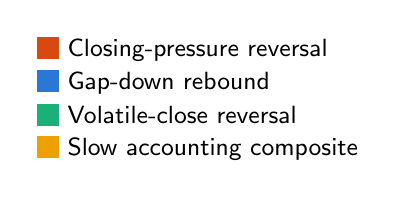
\begin{tikzpicture}
\foreach \c/\t [count=\i] in {famA/Closing-pressure reversal,famB/Gap-down rebound,famC/Volatile-close reversal,famD/Slow accounting composite}
  \node[anchor=west,font=\small] at (0,-0.42*\i) {{\color{\c}\rule[-1pt]{8pt}{8pt}}\ \t};
\end{tikzpicture}
\vfill
{\small\bfseries Abhinav Teja}\\
{\small\color{muted} Trexquant Alpha Generation Competition 2026 \textperiodcentered{} Trexsim (US equities, delay 0, Slow mode)}
\end{frame}

% ======================================================= 2. SUMMARY
\begin{frame}{Summary: four families, four best alphas}
\framesubtitle{Each family starts from one economic thesis; the highlighted alpha is the best of its family}
\vspace{4pt}
\renewcommand{\arraystretch}{1.35}
\scriptsize
\begin{tabular}{@{}P{2.9cm}P{4.0cm}lccccc@{}}
\toprule
\textbf{Family} & \textbf{Thesis (one line)} & \textbf{Best alpha} & \textbf{IR} & \textbf{TVR} & \textbf{DD} & \textbf{IR/$\sqrt{\text{TVR}}$} & \textbf{IR 17--21}\\
\midrule
\famtag{famA}{A. Closing-pressure reversal} & Late-day, price-insensitive flow pushes the close away from VWAP; the push reverts & \textbf{\#708808} & \textbf{.118} & .624 & \textbf{6.2} & .149 & \textbf{.145}\\
\famtag{famB}{B. Gap-down rebound} & A close pinned at the low after a gap-down is forced selling; liquidity providers are paid & \textbf{\#724045} & \textbf{.129} & .953 & 11.5 & .132 & .075\\
\famtag{famC}{C. Volatile-close reversal} & A close noisier than the open signals flow, not news, so the last-hour move fades & \textbf{\#685104} & .092 & .328 & 12.0 & .161 & .062\\
\famtag{famD}{D. Slow accounting composite} & Many weak, slow, low-correlated accounting premia add up to a steady signal & \textbf{\#716550} & .077 & \textbf{.036} & 12.4 & \textbf{.407} & \textbf{.139}\\
\bottomrule
\end{tabular}

\vspace{8pt}
\begin{columns}[T]
\column{0.5\textwidth}
\small
\begin{itemize}
\item All four best alphas are \textbf{submitted} and qualify on the portal.
\item Pairwise daily-PnL correlation between them: \textbf{0.06 to 0.48}.
\end{itemize}
\column{0.48\textwidth}
\scriptsize\color{muted}
IR = daily IR (\(\times 15.9\) for annual). TVR = daily turnover. DD = max drawdown (\%).
IR 17--21 = IR over 2017--2021, the most recent 5 years.
\textbf{Best in family} = highest recent (2017--21) IR among the family's submitted alphas, i.e.\ the most robust one.
\end{columns}
\end{frame}

% ======================================================= 3. PROCESS
\begin{frame}{Research process}
\framesubtitle{Thesis first; every alpha is a small, commented program with a written rationale and a source}
\vspace{6pt}
\begin{center}
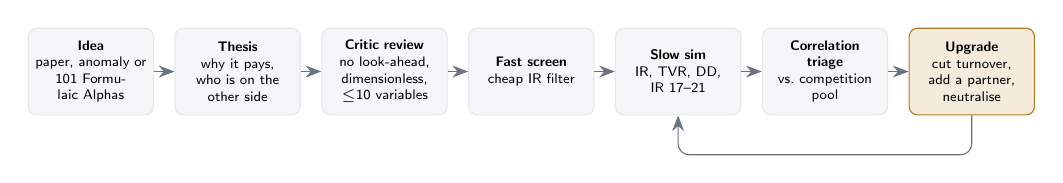
\begin{tikzpicture}[node distance=2.6mm,
  box/.style={draw=rule,fill=codebg,rounded corners=3pt,align=center,font=\tiny,minimum height=11mm,text width=14.5mm,inner sep=2pt},
  arr/.style={-{Stealth[length=2mm]},color=muted}]
\node[box](a){\textbf{Idea}\\paper, anomaly or\\101 Formulaic Alphas};
\node[box,right=of a](b){\textbf{Thesis}\\why it pays,\\who is on the\\other side};
\node[box,right=of b](c){\textbf{Critic review}\\no look-ahead,\\dimensionless,\\$\le$10 variables};
\node[box,right=of c](d){\textbf{Fast screen}\\cheap IR filter};
\node[box,right=of d](e){\textbf{Slow sim}\\IR, TVR, DD,\\IR 17--21};
\node[box,right=of e](f){\textbf{Correlation\\triage}\\vs.\ competition\\pool};
\node[box,right=of f,fill=gold!15,draw=gold](g){\textbf{Upgrade}\\cut turnover,\\add a partner,\\neutralise};
\foreach \x/\y in {a/b,b/c,c/d,d/e,e/f,f/g} \draw[arr](\x)--(\y);
\draw[arr,rounded corners] (g.south) -- ++(0,-5mm) -| (e.south);
\end{tikzpicture}
\end{center}
\vspace{4pt}
\begin{columns}[T]
\column{0.48\textwidth}
\textbf{\small What we learned}
\footnotesize
\begin{itemize}
\item Most daily IR in this universe comes from \textbf{short-term reversal}, so pure reversal ideas collide with the pool (correlation .78--.99).
\item Fast and Slow PnL of the same alpha correlate only \textbf{0.34}: we only trust Slow results.
\item The fix that worked: keep the thesis signal and add a \textbf{slow partner whose returns move against reversal} (low accruals: daily PnL correlation $\approx -0.2$). That cuts turnover and crowding without killing IR.
\end{itemize}
\column{0.48\textwidth}
\textbf{\small By the numbers}
\footnotesize
\begin{itemize}
\item \textbf{403} alphas simulated, \textbf{10} submitted.
\item 4 families, each traced below from the first version to the best alpha.
\item Every alpha documents its thesis, source and a comment on each line of code.
\end{itemize}
\end{columns}
\end{frame}

% ======================================================= A. THESIS
\begin{frame}[fragile]{\famtag{famA}{A. Closing-pressure reversal: thesis}}
\framesubtitle{Fade the gap between the close and the last-hour VWAP when the close was unusually busy}
\begin{columns}[T]
\column{0.45\textwidth}
\footnotesize
\textbf{Thesis}
\begin{itemize}
\item Index rebalancing, end-of-day hedging and fund flows trade \textbf{price-insensitively} in the last hour.
\item This pushes the close away from the hour's VWAP. Nobody is trading on news, so the push \textbf{reverts} over the next days.
\item The effect should be strongest on \textbf{busy closes} (many trades vs.\ the stock's own 20-day norm).
\end{itemize}
\textbf{Why add low accruals}
\begin{itemize}
\item Cash-backed earnings (Sloan) earn a slow premium whose daily PnL moves \emph{against} reversal, so the blend keeps the reversal IR with lower turnover and less overlap with crowded reversal alphas.
\end{itemize}
{\scriptsize\color{muted}Sources: Campbell, Grossman \& Wang (QJE 1993); Bogousslavsky \& Muravyev (2023), closing-auction price pressure; Sloan (The Accounting Review 1996).}
\column{0.53\textwidth}
\scriptsize\textbf{Best alpha \#708808 (simplified)}
\begin{lstlisting}
g    = ts_mean((close - vwap_last_hour)/vwap_last_hour, 5)
busy = cs_rank(trades_last_hour/ts_mean(trades_last_hour,20)) > 1.3
p1   = -cs_rank(g) * busy             # fade the gap on busy closes
hot  = cs_rank(volume/ts_mean(volume,20)) > 1.3
p2   = -(cs_rank(ts_mean(ret_last_hour,5)) + cs_rank(g)) * hot
rev  = cs_factorneut(p1 + p2, [size, volatility])
acc  = -cs_rank((net_income - cash_from_ops)/total_assets)
alpha = rev + 1.6 * acc               # reversal + low accruals
\end{lstlisting}
\vspace{2pt}
\textbf{First version \#673000: the pure thesis}
\begin{lstlisting}
g    = ts_mean((close - vwap_last_hour)/vwap_last_hour, 5)
busy = cs_rank(trades_last_hour/ts_mean(trades_last_hour,20)) > 1.3
alpha = -cs_rank(g) * busy
\end{lstlisting}
\end{columns}
\end{frame}

% ======================================================= A. EVOLUTION
\begin{frame}{\famtag{famA}{A. Closing-pressure reversal: from thesis to best alpha}}
\framesubtitle{IR .083 $\to$ .118, drawdown halved (12.5 $\to$ 6.2), recent IR .085 $\to$ .145}
\scriptsize
\renewcommand{\arraystretch}{1.2}
\begin{tabular}{@{}llP{6.0cm}ccccc@{}}
\toprule
& \textbf{Alpha} & \textbf{Change} & \textbf{IR} & \textbf{TVR} & \textbf{DD} & \textbf{IR/$\sqrt{\text{TVR}}$} & \textbf{IR 17--21}\\
\midrule
1 & \#673000 & Pure thesis: fade close-vs-VWAP gap on busy closes. Pool correlation .78 & .083 & 1.047 & 12.5 & .081 & .085\\
2 & \#705948 & + R\&D, buybacks, low accruals; size-neutral; book held for the week & .080 & .248 & 11.7 & .161 & .069\\
3 & \#707365 & Accruals weight 1.5$\times$ (submitted) & .085 & .226 & 11.6 & \textbf{.179} & .077\\
\best{famA} 4 & \textbf{\#708808} \badge{BEST} & Two late-day pressure legs, size/vol-neutral, + 1.6$\times$ low accruals (submitted) & \textbf{.118} & .624 & \textbf{6.2} & .149 & \textbf{.145}\\
\bottomrule
\end{tabular}

\vspace{3pt}
{\centering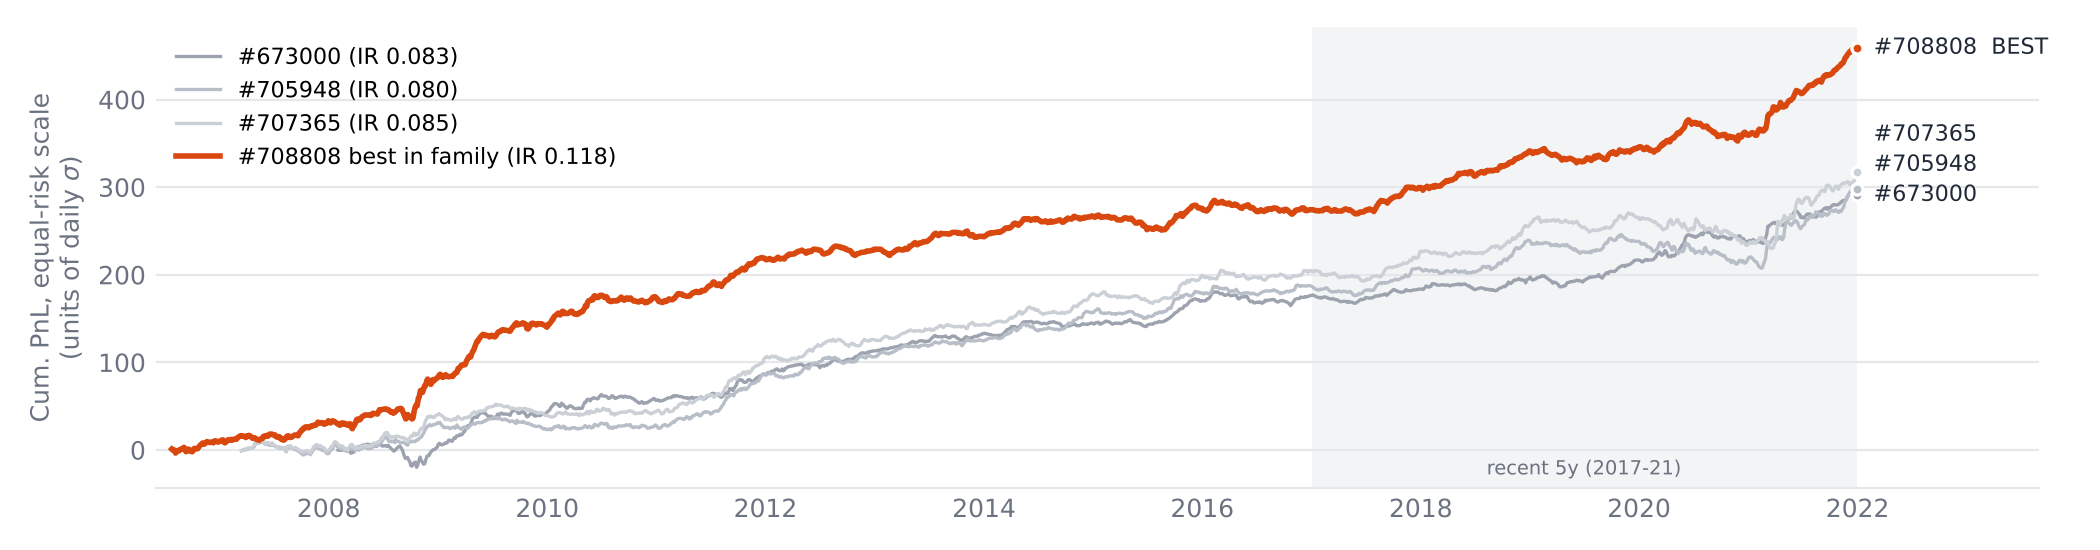
\includegraphics[width=\linewidth]{charts/famA.png}\par}\vspace{-1pt}
{\tiny\color{muted}Curves traced from the Trexsim PnL charts and scaled to equal risk, so a steeper line means a higher IR. Shaded: the recent 5 years (2017--21) used to pick the best alpha.}\par
\end{frame}

% ======================================================= B. THESIS
\begin{frame}[fragile]{\famtag{famB}{B. Gap-down rebound: thesis}}
\framesubtitle{Buy stocks that opened down and closed pinned at the day's low (Alpha \#54, adapted)}
\begin{columns}[T]
\column{0.45\textwidth}
\footnotesize
\textbf{Thesis}
\begin{itemize}
\item A stock that \textbf{gaps down} and closes \textbf{at its low} was sold all day: margin calls, stop-losses, forced selling.
\item Short-term reversal is the return to \textbf{providing liquidity}; it is largest when sellers are impatient.
\item The \((\text{open}/\text{close})^5\) term scales the bet by the size of the drop.
\end{itemize}
\textbf{Why add a slow partner}
\begin{itemize}
\item The raw formula is public: our standalone version was \textbf{.995} correlated with an alpha already in the pool.
\item A slow balance-sheet partner (short-term liabilities/assets) changes the PnL path and gave the best recent IR.
\end{itemize}
{\scriptsize\color{muted}Sources: Kakushadze, ``101 Formulaic Alphas'' (2016), arXiv:1601.00991; Nagel, ``Evaporating Liquidity'' (RFS 2012); Sloan (1996).}
\column{0.53\textwidth}
\scriptsize\textbf{Best alpha \#724045}
\begin{lstlisting}
loc  = (low - close)/(low - high - 0.001*close)  # 0 = closed at low
b    = cs_zscore(-loc * (open/close)**5)          # Alpha #54
p_cl = cs_zscore(cs_rank(current_liabilities/total_assets))
alpha = b + 1.5 * p_cl
\end{lstlisting}
\vspace{2pt}
\textbf{First submission \#715966}
\begin{lstlisting}
acc  = cs_zscore(-cs_rank((net_income - cash_from_ops)/total_assets))
alpha = b + 1.5 * acc                             # low accruals partner
\end{lstlisting}
\vspace{2pt}
\textbf{First version (standalone Alpha \#54)}
\begin{lstlisting}
alpha = -loc * (open/close)**5
\end{lstlisting}
\end{columns}
\end{frame}

% ======================================================= B. EVOLUTION
\begin{frame}{\famtag{famB}{B. Gap-down rebound: from thesis to best alpha}}
\framesubtitle{Highest IR of all families; recent IR .015 $\to$ .075 after adding slow partners}
\scriptsize
\renewcommand{\arraystretch}{1.2}
\begin{tabular}{@{}llP{6.0cm}ccccc@{}}
\toprule
& \textbf{Alpha} & \textbf{Change} & \textbf{IR} & \textbf{TVR} & \textbf{DD} & \textbf{IR/$\sqrt{\text{TVR}}$} & \textbf{IR 17--21}\\
\midrule
1 & Alpha \#54 & Standalone formula. Pool correlation .995: already taken & .112 & 1.381 & -- & .095 & .015\\
2 & \#715966 & + 1.5$\times$ low accruals (submitted) & \textbf{.137} & .994 & \textbf{10.6} & \textbf{.137} & .064\\
\best{famB} 3 & \textbf{\#724045} \badge{BEST} & Partner from grid search: current liabilities/assets at 1.5$\times$ (submitted) & .129 & .953 & 11.5 & .132 & \textbf{.075}\\
\bottomrule
\end{tabular}

\vspace{3pt}
{\centering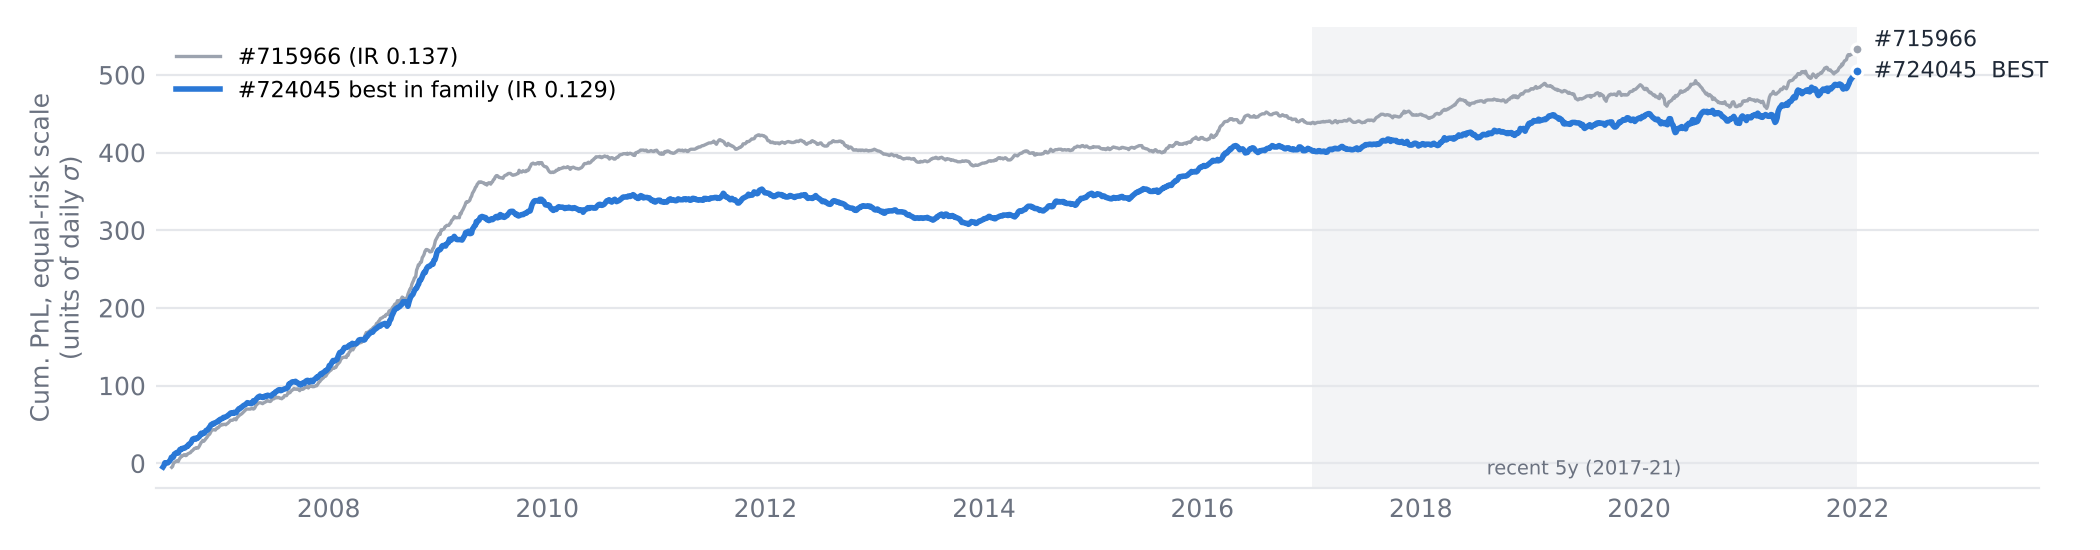
\includegraphics[width=\linewidth]{charts/famB.png}\par}\vspace{-1pt}
{\tiny\color{muted}Curves traced from the Trexsim PnL charts and scaled to equal risk, so a steeper line means a higher IR. Shaded: the recent 5 years (2017--21) used to pick the best alpha.}\par
\vspace{2pt}
{\scriptsize\color{muted}Honest read: most PnL came in 2006--09, when liquidity provision pays most. \#724045 beats \#715966 on recent IR and pool correlation (.77 vs .83); the two are .84 correlated.}
\end{frame}

% ======================================================= C. THESIS
\begin{frame}[fragile]{\famtag{famC}{C. Volatile-close reversal: thesis}}
\framesubtitle{Fade the last-hour move only where the close was more volatile than the open}
\begin{columns}[T]
\column{0.45\textwidth}
\footnotesize
\textbf{Thesis}
\begin{itemize}
\item News is absorbed at the \textbf{open}; a close that is \textbf{noisier than the open} is driven by flow (hedging, rebalancing, liquidations), not information.
\item Flow-driven moves revert. So we fade the 5-day last-hour return only for stocks whose last hour is unusually volatile relative to their first hour.
\item This works best when markets are stressed: a \textbf{crisis alpha} that diversifies the other families.
\end{itemize}
\textbf{Why add slow partners}
\begin{itemize}
\item Less common slow premia (stock-based pay, buybacks, free-cash-flow yield, low accruals) carry most of the risk, so the mix differs from crowded reversal and fundamental alphas.
\end{itemize}
{\scriptsize\color{muted}Sources: Bogousslavsky \& Muravyev (2023); Nagel (RFS 2012); Pontiff \& Woodgate (JF 2008); Lakonishok, Shleifer \& Vishny (JF 1994); Sloan (1996).}
\column{0.53\textwidth}
\scriptsize\textbf{Best alpha \#685104 (simplified)}
\begin{lstlisting}
late = cs_rank(ts_mean(std_ret_last_hour /
               (std_ret_first_hour + 1e-4), 5)) > 1.5
r  = -cs_rank(ts_mean(ret_last_hour, 5)) * late  # fade flow
k1 = cs_rank(stock_based_comp / mktcap)          # intangibles
k2 = -cs_rank(shsout/ts_delay(shsout,250) - 1)   # buybacks
k3 = cs_rank(free_cash_flow / mktcap)            # FCF yield
k4 = -cs_rank((net_income - cash_from_ops)/total_assets)
alpha = r + 2 * (k1 + k2 + k3 + k4)
\end{lstlisting}
\vspace{2pt}
\textbf{Upgrade path}
\begin{lstlisting}
#678911  r + 2*(k1+k2+k3)       first version
#684336  r + 3*(k1+k2+k3)       our first submission
#685104  r + 2*(k1+k2+k3+k4)    + low accruals  -> BEST
\end{lstlisting}
\end{columns}
\end{frame}

% ======================================================= C. EVOLUTION
\begin{frame}{\famtag{famC}{C. Volatile-close reversal: from thesis to best alpha}}
\framesubtitle{Drawdown 17.7 $\to$ 12.0, turnover .54 $\to$ .33, IR .075 $\to$ .092}
\scriptsize
\renewcommand{\arraystretch}{1.2}
\begin{tabular}{@{}llP{6.0cm}ccccc@{}}
\toprule
& \textbf{Alpha} & \textbf{Change} & \textbf{IR} & \textbf{TVR} & \textbf{DD} & \textbf{IR/$\sqrt{\text{TVR}}$} & \textbf{IR 17--21}\\
\midrule
1 & \#678911 & Volatile-close reversal + stock pay, buybacks, FCF yield at 2$\times$ & .075 & .540 & 17.7 & .102 & .034\\
2 & \#684336 & Slow weight 3$\times$ (our first submission) & .073 & .486 & 17.7 & .105 & .031\\
\best{famC} 3 & \textbf{\#685104} \badge{BEST} & + low accruals as 4th slow leg, 2$\times$ (submitted) & \textbf{.092} & \textbf{.328} & \textbf{12.0} & \textbf{.161} & \textbf{.062}\\
\bottomrule
\end{tabular}

\vspace{3pt}
{\centering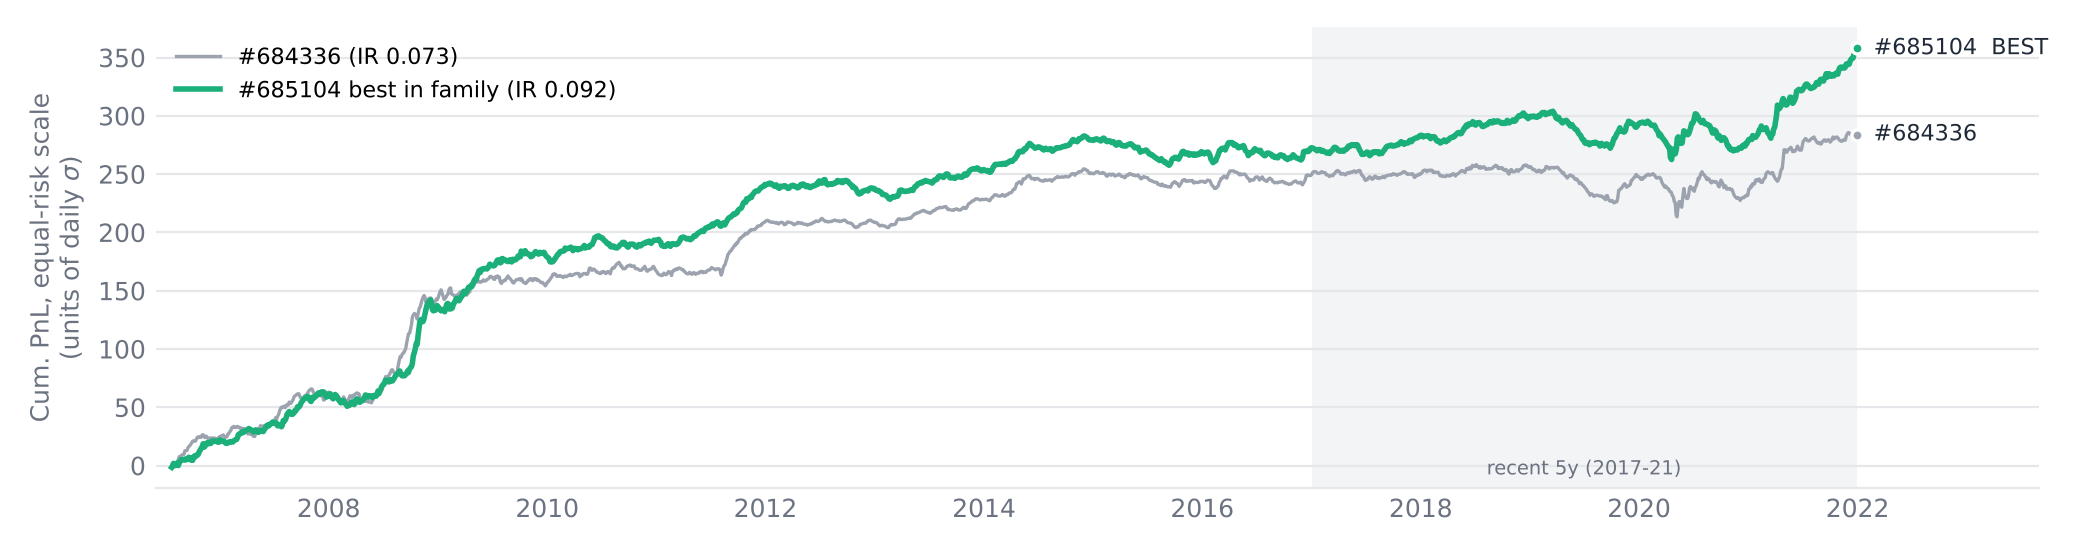
\includegraphics[width=\linewidth]{charts/famC.png}\par}\vspace{-1pt}
{\tiny\color{muted}Curves traced from the Trexsim PnL charts and scaled to equal risk, so a steeper line means a higher IR. Shaded: the recent 5 years (2017--21) used to pick the best alpha.}\par
\vspace{2pt}
{\scriptsize\color{muted}Honest read: gains cluster in stressed markets (2008, 2011, 2020--21) and are flat in calm 2014--19, as the crisis-alpha thesis predicts.}
\end{frame}

% ======================================================= D. THESIS
\begin{frame}[fragile]{\famtag{famD}{D. Slow accounting composite: thesis}}
\framesubtitle{Weak, slow, low-correlated balance-sheet premia combined into one steady signal}
\begin{columns}[T]
\column{0.45\textwidth}
\footnotesize
\textbf{Thesis}
\begin{itemize}
\item Each accounting ratio (item/assets) is a \textbf{weak} predictor (IR .03--.05) but changes only quarterly, so turnover is tiny.
\item The ratios are \textbf{weakly related}, so averaging diversifies their noise: higher IR at the same turnover, so a very high IR/$\sqrt{\text{TVR}}$.
\item Long cash-backed earnings, operating-liability funding, older asset bases; short goodwill-heavy (acquisitive) firms.
\end{itemize}
\textbf{Guarding against data-mining}
\begin{itemize}
\item Every leg's sign was checked to hold \textbf{out of sample (2017--21)} before it was included.
\end{itemize}
{\scriptsize\color{muted}Sources: Sloan (1996); Green, Hand \& Zhang (RFS 2017); Cooper, Gulen \& Schill (JF 2008); Pontiff \& Woodgate (JF 2008); Novy-Marx (JFE 2013).}
\column{0.53\textwidth}
\scriptsize\textbf{Best alpha \#716550}
\begin{lstlisting}
ta = ts_fill(total_assets)
cl = cs_rank(current_liabilities / ta)      # operating funding
ar = cs_rank(accounts_receivable / ta)      # receivables
gw = -cs_rank(goodwill / ta)                # short acquirers
ad = cs_rank(accumulated_depreciation / ta) # older assets
oc = cs_rank(other_current_assets / ta)
acc = -cs_rank((net_income - cash_from_ops) / ta)
alpha = cl + ar + gw + ad + oc + acc        # equal weight
\end{lstlisting}
\vspace{2pt}
\textbf{Upgrade path}
\begin{lstlisting}
#679831  low accruals + low asset growth          (2 premia)
#685741  7 classic premia: accruals, issuance,
         FCF, asset growth, R&D, gross profit, SBC
#716550  balance-sheet composition + accruals  -> BEST
\end{lstlisting}
\end{columns}
\end{frame}

% ======================================================= D. EVOLUTION
\begin{frame}{\famtag{famD}{D. Slow accounting composite: from thesis to best alpha}}
\framesubtitle{IR/$\sqrt{\text{TVR}}$ .30 $\to$ .41, turnover .036, strongest recent performance of all families}
\scriptsize
\renewcommand{\arraystretch}{1.2}
\begin{tabular}{@{}llP{6.0cm}ccccc@{}}
\toprule
& \textbf{Alpha} & \textbf{Change} & \textbf{IR} & \textbf{TVR} & \textbf{DD} & \textbf{IR/$\sqrt{\text{TVR}}$} & \textbf{IR 17--21}\\
\midrule
1 & \#679831 & Low accruals + low asset growth & .067 & .051 & 11.2 & .298 & .095\\
2 & \#685741 & 7-premium composite (submitted) & \textbf{.083} & .051 & \textbf{11.1} & .366 & .076\\
\best{famD} 3 & \textbf{\#716550} \badge{BEST} & Balance-sheet composition (5 items/assets) + low accruals (submitted) & .077 & \textbf{.036} & 12.4 & \textbf{.407} & \textbf{.139}\\
\bottomrule
\end{tabular}

\vspace{3pt}
{\centering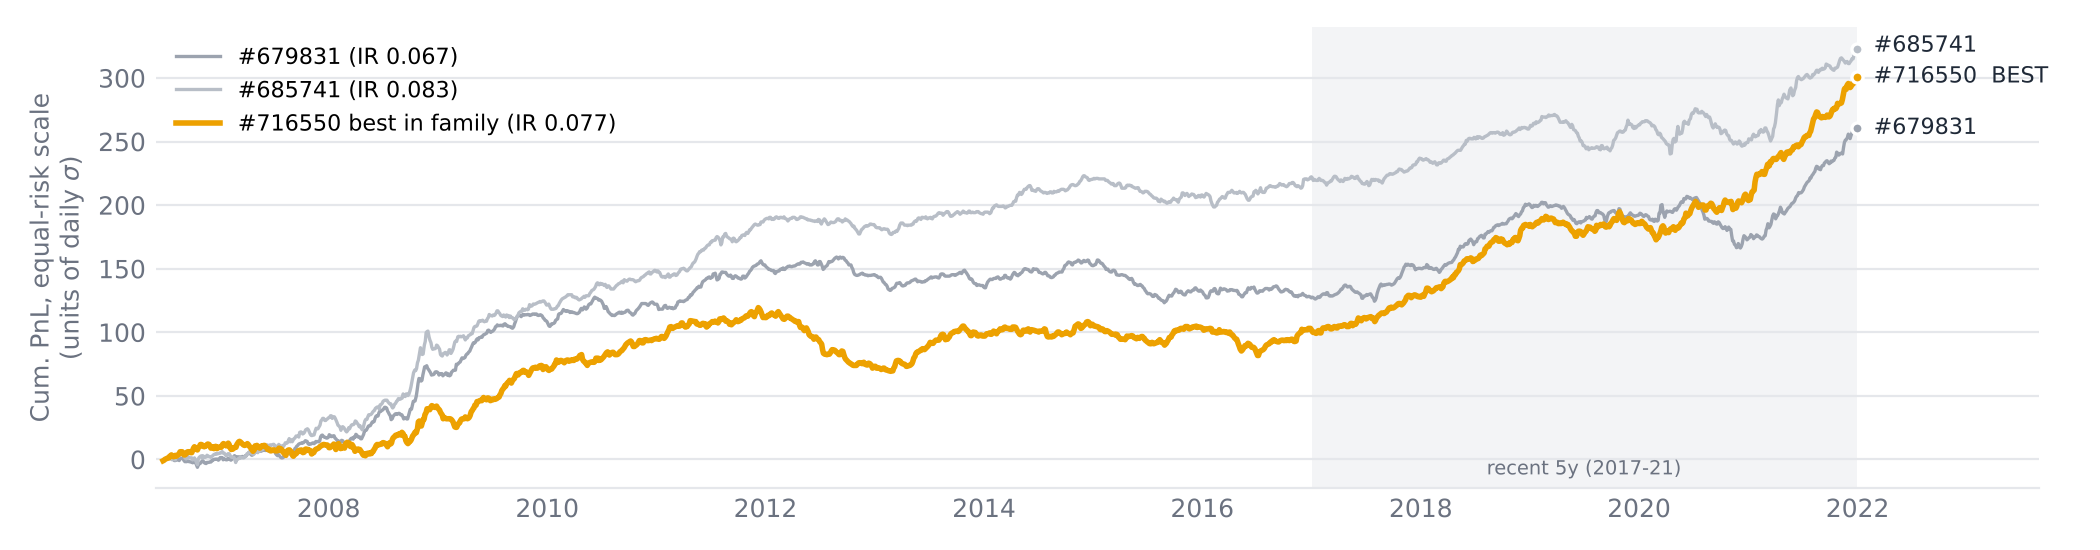
\includegraphics[width=\linewidth]{charts/famD.png}\par}\vspace{-1pt}
{\tiny\color{muted}Curves traced from the Trexsim PnL charts and scaled to equal risk, so a steeper line means a higher IR. Shaded: the recent 5 years (2017--21) used to pick the best alpha.}\par
\vspace{2pt}
{\scriptsize\color{muted}\#716550 beats \#685741 (higher full-period IR) on recent IR (almost 2$\times$), turnover and pool correlation (.53 vs .79).}
\end{frame}

% ======================================================= 12. DIVERSIFICATION
\begin{frame}{Diversification across families and takeaways}
\framesubtitle{The four best alphas make money at different times}
\begin{columns}[T]
\column{0.56\textwidth}
\centering
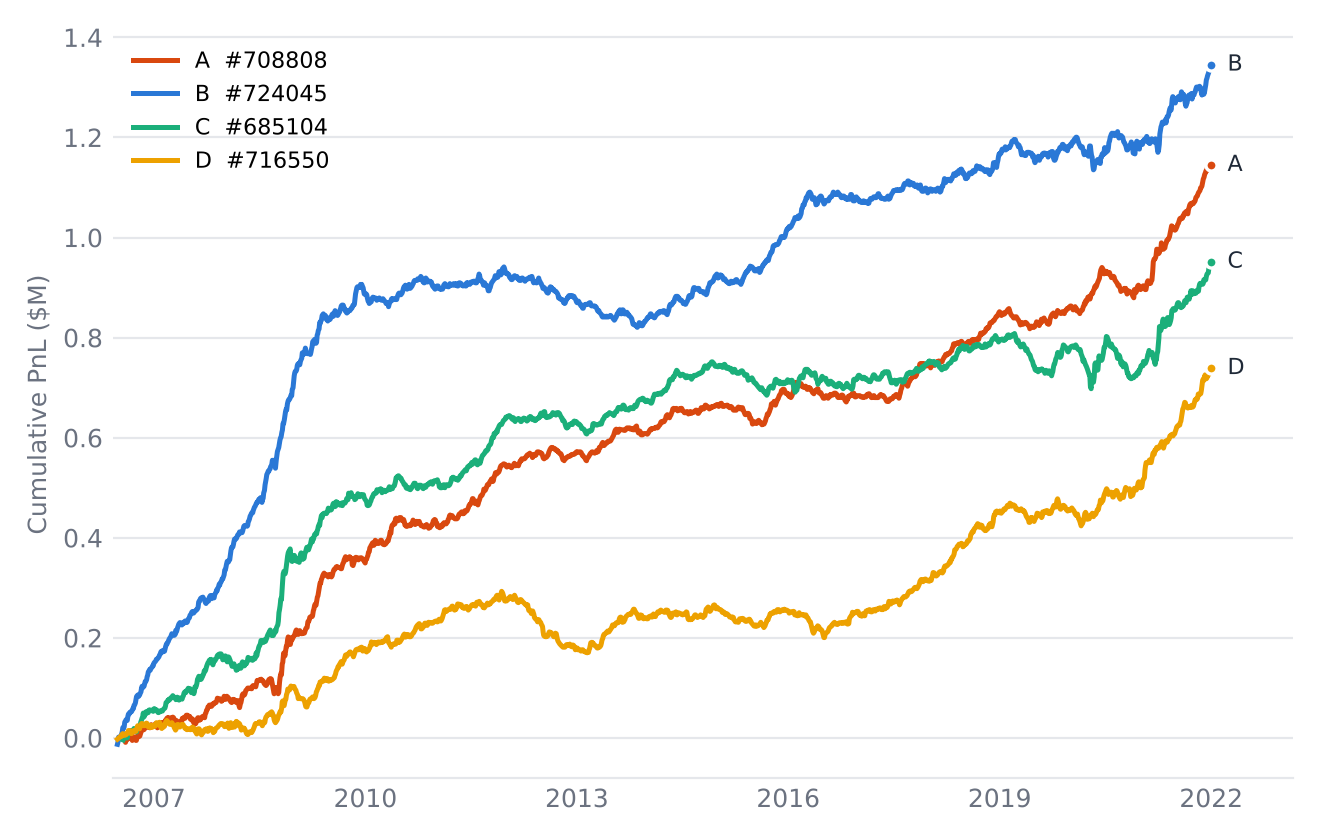
\includegraphics[width=\linewidth]{charts/finals.png}\\
{\tiny\color{muted}Cumulative PnL in \$M of the four best alphas, 2006--2021 (traced from the Trexsim PnL charts).}
\column{0.42\textwidth}
\textbf{\small Daily PnL correlation (2020--21)}\\[3pt]
\scriptsize
\renewcommand{\arraystretch}{1.25}
\begin{tabular}{@{}lcccc@{}}
\toprule
 & {\color{famA}\rule[-1pt]{6pt}{6pt}}\,\textbf{A} & {\color{famB}\rule[-1pt]{6pt}{6pt}}\,\textbf{B} & {\color{famC}\rule[-1pt]{6pt}{6pt}}\,\textbf{C} & {\color{famD}\rule[-1pt]{6pt}{6pt}}\,\textbf{D}\\
\midrule
{\color{famA}\rule[-1pt]{6pt}{6pt}}\,\textbf{A} \#708808 & 1 & .20 & .48 & .25\\
{\color{famB}\rule[-1pt]{6pt}{6pt}}\,\textbf{B} \#724045 & .20 & 1 & .06 & .19\\
{\color{famC}\rule[-1pt]{6pt}{6pt}}\,\textbf{C} \#685104 & .48 & .06 & 1 & .17\\
{\color{famD}\rule[-1pt]{6pt}{6pt}}\,\textbf{D} \#716550 & .25 & .19 & .17 & 1\\
\bottomrule
\end{tabular}

\vspace{4pt}
\textbf{\small Takeaways}
\begin{itemize}\scriptsize
\item Every best alpha starts from a \textbf{clear economic thesis} with a named counterparty.
\item The upgrade that worked: keep the thesis signal, add a \textbf{slow partner} that moves against reversal; it cuts turnover and crowding.
\item The four families are \textbf{largely uncorrelated} (max .48), so together they form a diversified book.
\end{itemize}
\vspace{4pt}
{\scriptsize\color{muted}Code, theses and the full log of 403 simulations:\\ \url{https://github.com/abhinavteja2005/trexquant-alpha-research}}
\end{columns}
\end{frame}

\end{document}
